\documentclass{article}
\usepackage[utf8x]{inputenc} % Включаем поддержку UTF8  
\usepackage[russian]{babel}  % Включаем пакет для поддержки русского языка 	
\usepackage{amsmath}

\usepackage{graphicx}
\graphicspath{{}}
\DeclareGraphicsExtensions{.png}

\begin{document}
	\begin{titlepage}
		\begin{center}
		\large
		Государственное образовательное учреждение высшего профессионального образования\\
		“Московский государственный технический университет имени Н.Э.Баумана”
		\vspace{0.25cm}
		
		
		\textsc{Дисциплина: Анализ алгоритмов}\\[5mm]
		\vfill
			
		\textsc{Лабораторная работа № 1}\\[5mm]
		
		{\LARGE Алгоритм Левенштейна}
		\bigskip
		
			
		Бутолин Александр Алексеевич\\
		Студент группы ИУ7-52
		\vfill		
		
		\end{center}
		\begin{center}
			2018 г.
		\end{center}
	\end{titlepage}

	

\begin{center}
	\textbf{Введение}
	\label{sec:intro}
\end{center}

В настоящее время каждый день пользователи компьютеров сталкиваются с вводом текста: поисковые запросы, сообщения в социальных сетях, написание отчетов и докладов. Пользователи могут ошибаться в словах, и компьютер должен подсказать, как исправить ошибку. Данная задача решается с использованием алгоритмов, определяющих степень различия двух строк. Для этой цели математик Владимир Иосифович Левенштейн ввел понятие расстояния между двумя строками и разработал алгоритм нахождения этого расстояния.

В лабораторной работе рассматривается задача нахождения расстояния Левенштейна и Дамерау-Левенштейна между двумя строками..

Цель работы: изучение метода динамического программирования на материале алгоритмов Левенштейна и Дамерау-Левенштейна.

Задачи работы:

\begin{enumerate}
	\item {Изучение алгоритмов Левенштейна и Дамерау-Левенштейна нахождения расстояния между строками;}
	\item {Сравнение матричной и рекурсивной реализаций выбранного алгоритма определения расстояния между строками по затрачиваемым ресурсам (времени и памяти)};
	\item {Экспериментальное подтверждение различий во временной эффективности рекурсивной и нерекурсивной реализаций выбранного алгоритма определения расстояния между строками при помощи разработанного программного обеспечения на материале замеров процессорного времени выполнения реализации на варьирующихся длинах строк;}
	\item {Описание и обоснование полученных результатов в отчете о выполненной лабораторной работе, выполненного как расчётно-пояснительная записка к работе.}
\end{enumerate}

\newpage
\section{Аналитический раздел}
\label{sec:analitics}

Термин «редакционное расстояние» (или «расстояние Левенштейна») был введен советским математиком Владимиром Иосифовичем Левенштейном в начале второй половины 20 века.

Расстояние Левенштейна между двумя строками - это минимальное количество операций вставки одного символа, удаления одного символа и замены одного символа на другой, необходимых для превращения одной строки в другую. При этом все три операции обладают так называемым штрафом или ценой, которая может варьироваться в зависимости от различных факторов

Если к списку разрешённых операций добавить транспозицию (два соседних символа меняются местами), получается расстояние Дамерау — Левенштейна.

В этих методах нахождения расстояния Левенштейна и Дамерау-Левенштейна стоимость операций замены, вставки и удаления принята за единицу, однако последний учитывает транспозицию двух символов как еще одну операцию стоимостью 1. Ниже приведено более подробное описание этих алгоритмов с указанием формул для вычисления расстояния.

\subsection{Описание алгоритмов}
\label{sec:analitics:alg}

Пусть S1 и S2 – строки длины i и j соответственно, для которых необходимо найти расстояние Левенштейна. Здесь и далее полагается, что символы в строках нумеруются начиная с 1. Тогда алгоритм можно описать формулой (1).

\begin{equation*}
D(S1[i..1],S2[1..j]) = 
 \begin{cases}
	i,  \mbox{  если  }  𝑗=0\\
      j,  \mbox{  если  } 𝑖=0\\
	\mbox{min}(𝐷(𝑆1[1..𝑖−1],𝑆2[1..𝑗])+1,\\ 
				𝐷(𝑆1[1..𝑖],𝑆2[1..𝑗−1])+1, \\
				𝐷(𝑆1[1..𝑖−1],𝑆2[1..𝑗−1])+𝑚(𝑆1[𝑖−1],𝑆2[𝑗−1])), \mbox{  иначе}
\end{cases}
\end{equation*}

где m находится из формулы (2), как:

\begin{equation*}
𝑚(𝑆1[𝑖−1],𝑆2[𝑗−1] = 
 \begin{cases}
	0,  \mbox {  если  𝑆1[𝑖−1]= 𝑆2[𝑗−1]  } \\
	1, \mbox {  иначе  }
\end{cases}
\end{equation*}

Алгоритм Дамерау-Левенштейна является модификацией исходного алгоритма Левенштейна. В отличии от исходного алгоритма, он учитывает перестановку двух соседних символов местами – транспозицию, которая также имеет стоимость 1.

Расстояние Дамерау-Левенштейна для строк S1 и S2 можно найти по формуле (3).

\begin{equation*}
𝐷(𝑆1[1..𝑖],𝑆2[1..𝑗]) = 
 \begin{cases}
	i,  \mbox{  если  }  𝑗=0\\
      j,  \mbox{  если  }  𝑖=0\\
	\mbox{min}(𝐷(𝑆1[1..𝑖−1],𝑆2[1..𝑗])+1,\\ 
		𝐷(𝑆1[1..𝑖],𝑆2[1..𝑗−1])+1,\\ 
		𝐷(𝑆1[1..𝑖−1],𝑆2[1..𝑗−1])+𝑚(𝑆1[𝑖−1],𝑆2[𝑗−1]),\\
		𝐷(𝑆1[1..𝑖−2],𝑆2[1..𝑗−2]), \mbox {  если 𝑖,𝑗>1 и 𝑆1[𝑖−1]=𝑆2[𝑗] и 𝑆1[𝑖]=𝑆2[𝑗−1]  } \\
	\mbox{min}(𝐷(𝑆1[1..𝑖−1],𝑆2[1..𝑗])+1,\\
		𝐷(𝑆1[1..𝑖],𝑆2[1..𝑗−1])+1, \\
		𝐷(𝑆1[1..𝑖−1],𝑆2[1..𝑗−1])+𝑚(𝑆1[𝑖−1],𝑆2[𝑗−1])), \mbox {иначе}		
\end{cases}
\end{equation*}

где m вычисляется по формуле (2).

\newpage
\section{Конструкторская часть}
\label{sec:construct}

Алгоритмы Левенштейна и Дамерау-Левенштейна можно реализовать как рекурсивно, так и нерекурсивно. Ниже представлены три схемы для этих алгоритмов, также для расстояния Левенштейна представлены как рекурсивная, так и нерекурсивная реализации и приведен их сравнительный анализ

\subsection{Разработка Алгоритмов}
\label{sec:analitics:alg}

В соответствии с описанием методов поиска расстояния Левенштейна и Дамерау-Левенштейна, представленным в аналитическом разделе данной работы, были построены схемы трех выбранных реализаций указанных алгоритмов.

На рисунках 2.1.1., 2.1.2. и 2.1.3. представлены нерекурсивная и рекурсивная реализации алгоритма Левенштейна и нерекурсивная реализация алгоритма Дамерау-Левенштейна соответственно.

\small 
	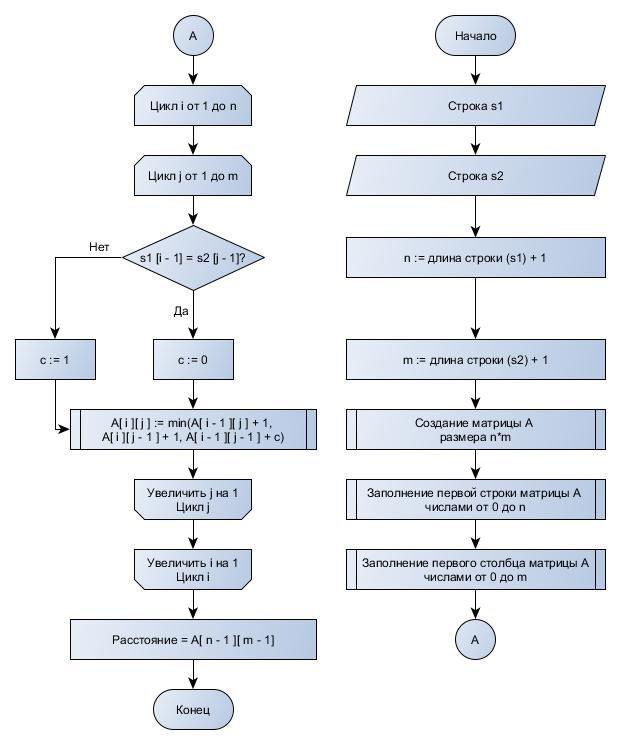
\includegraphics[width=10cm]{a}\\
	Рисунок 2.1.1. – схема нерекурсивного алгоритма поиска расстояния Левенштейна
	\\
	\\
\\
	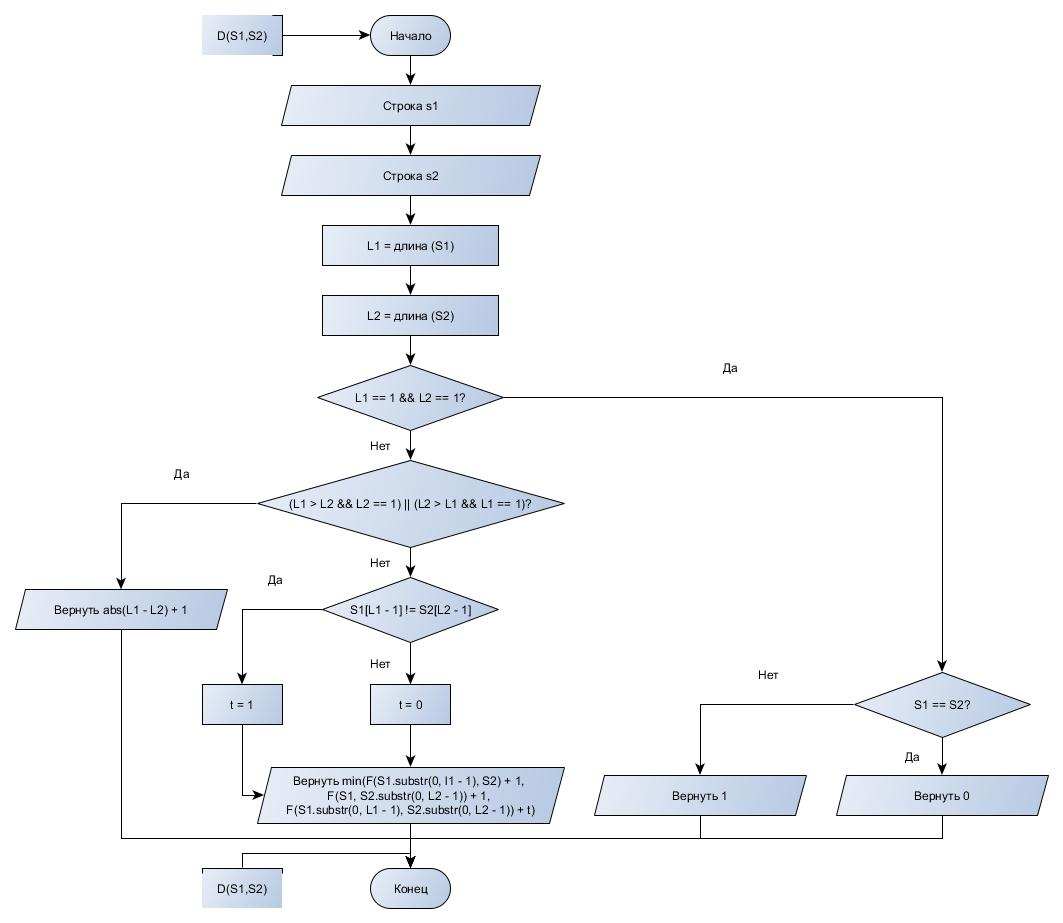
\includegraphics[width=13cm]{c}\\
	Рисунок 2.1.2. – схема рекурсивного алгоритма поиска расстояния Левенштейна
	\\
\\
	\\	
	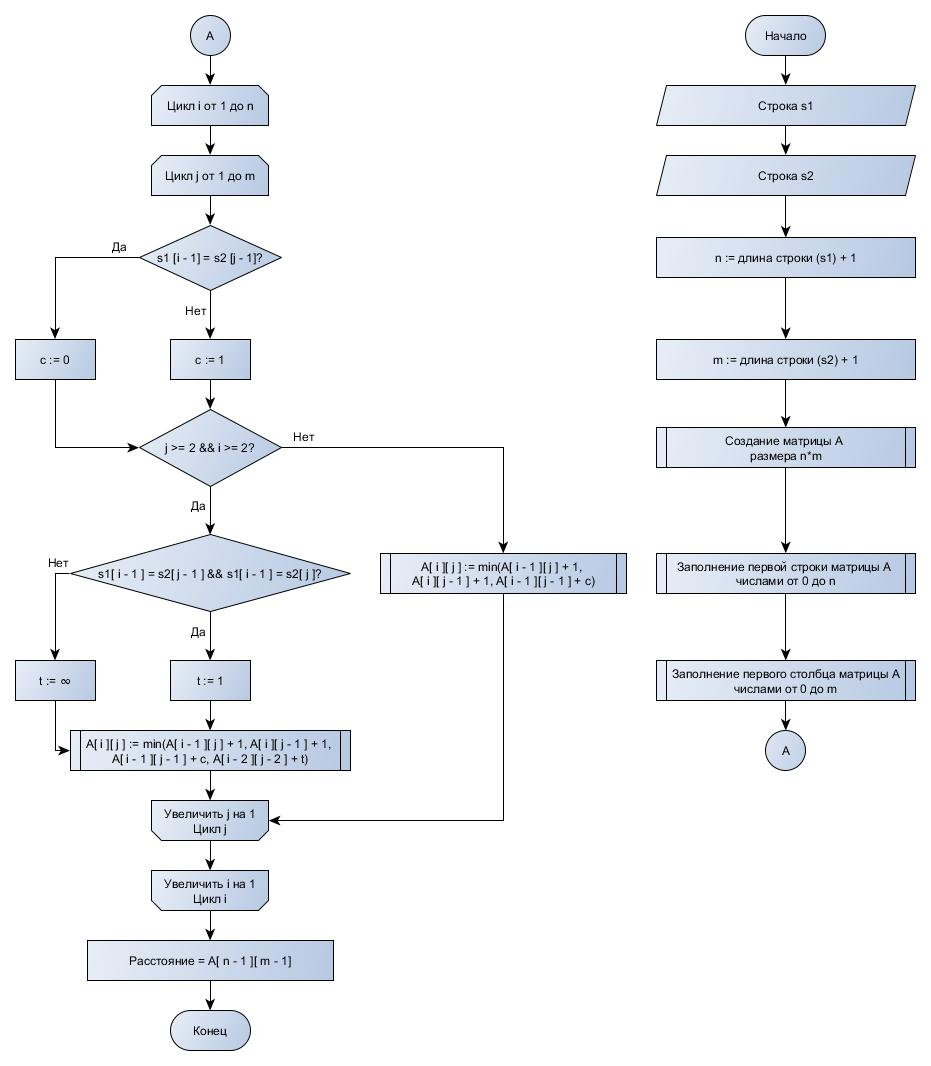
\includegraphics[width=11cm]{b}\\
	Рисунок 2.1.3. – схема нерекурсивного алгоритма поиска расстояния Дамерау-Левенштейна
\normalsize

\newpage
\subsection{Вывод}
\label{sec:analitics:construct}

В данном разделе в соответствии с формулами алгоритмов Левенштейна и Дамерау-Левенштейна, приведенными в аналитической части работы, были разработаны схемы для итерационных реализаций указанных алгоритмов и рекурсивной реализации алгоритма Левенштейна. Для последнего также было приведено сравнение рекурсивной и итеративной реализации, из которого можно заключить, что рекурсивная реализация алгоритма Левенштейна должна сильно уступать нерекурсивной по количеству вычислений и числу хранимых во время выполнения данных, а, следовательно, и по памяти, и по времени.

\newpage
\section{Технологическая часть}
\label{sec:technologicalt}

В технологическом разделе представлены требования к разрабатываемому программному обеспечению, средства, использованные в процессе разработки для реализации поставленных задач, а также листинг кода программы.

\subsection{Требования к программному обеспечению}
\label{sec:technologicalt:requirements}

Программное обеспечение должно реализовывать два алгоритма нахождения расстояния между двумя строками – алгоритм Левенштейна и алгоритм Дамерау-Левенштейна, причем алгоритм Левенштейна должен быть реализован как рекурсивным, так и нерекурсивным способом. Пользователь должен иметь возможность проводить как единичный замер расстояния для выбранной пары строк, так и возможность сравнить скорость работы этих алгоритмов.

Разработанное ПО должно предоставлять возможность замеров процессорного времени выполнения реализации каждого алгоритма. Требуется провести замеры для варьирующихся длин строк (длины сравниваемых строк полагать одинаковыми): не менее чем от 100 до 1000 с шагом 100. Один эксперимент ставится не менее 100 раз, результат одного эксперимента рассчитывается как средний из результатов проведенных испытаний с одинаковыми входными данными.


\subsection{Средства реализации}
\label{sec:technologicalt:software}

Для реализации поставленной задачи был использован язык программирования C++.
Для измерения процессорного времени была использована ассемблерная команда rdtsc.

\subsection{Листинг кода}
\label{sec:technologicalt:code}
Ниже приведен листинг кода для трех реализованных алгоритмов – итерационного и рекурсивного алгоритма 
Левенштейна и нерекурсивного алгоритма Дамерау-Левенштейна.\\

\newpage
\small \textbf{Листинг 1. Код нерекурсивной реализации алгоритма Левенштейна:} \normalsize

\begin{verbatim}
int levenshtein_distance(const string & src, const string & dst)
{
       const int m = src.size();
       const int n = dst.size();

       if (m == 0)
             return n;
       if (n == 0)
             return m;

       vector <vector <int>> matrix(m + 1);

       for (int i = 0; i <= m; i++)
       {
             matrix[i].resize(n + 1);
             matrix[i][0] = i;
       }

       for (int i = 0; i <= n; i++)
       {
             matrix[0][i] = i;
       }

       int above_cell, left_cell, diagonal_cell, cost;

       for (int i = 1; i <= m; i++)
       {
            for (int j = 1; j <= n; j++)
            {
                   cost = src[i - 1] == dst[j - 1] ? 0 : 1;
                   above_cell = matrix[i - 1][j];
                   left_cell = matrix[i][j - 1];
                   diagonal_cell = matrix[i - 1][j - 1];
                   matrix[i][j] = min_3(above_cell + 1, left_cell + 1,
                                                          diagonal_cell + cost);
             }
        }

      return matrix[m][n];
}
\end{verbatim}


\newpage
\small \textbf{Листинг 2. Код нерекурсивной реализации алгоритма Дамерау - Левенштейна:} \normalsize
\begin{verbatim}
int damerau_levenshtein_distance(const string & src, const string & dst)
{
      const int m = src.size();
      const int n = dst.size();

      if (m == 0)
             return n;
      if (n == 0)
             return m;

      vector <vector <int>> matrix(m + 1);

      for (int i = 0; i <= m; i++)
      {
             matrix[i].resize(n + 1);
             matrix[i][0] = i;
      }

      for (int i = 0; i <= n; i++)
      {
             matrix[0][i] = i;
      }

      int above_cell, left_cell, diagonal_cell, cost_replacement;
      int cost_transposition, transposition_cell, dem_len;

      for (int i = 1; i <= m; i++)
      {
             for (int j = 1; j <= n; j++)
             {
                   cost_replacement = src[i - 1] == dst[j - 1] ? 0 : 1;
                   above_cell = matrix[i - 1][j];
                   left_cell = matrix[i][j - 1];
                   diagonal_cell = matrix[i - 1][j - 1];


                   cost_transposition = 2;
                   if (i >= 2 and j >= 2)
                   {
                          transposition_cell = matrix[i - 2][j - 2];
                          cost_transposition = src[i - 1] == dst[j - 2] and 
                                                   src[i - 2] == dst[j - 1] ? 1 : 2;
                   }

                   if (cost_transposition == 1)
                   {
                         matrix[i][j] = min_3(min(above_cell + 1, left_cell + 1), 
                                                diagonal_cell + cost_replacement, 
                                                  transposition_cell + cost_transposition);
                    }
                         else if (cost_transposition == 2)
                    {
                         matrix[i][j] = min_3(above_cell + 1, left_cell + 1,
                                                  diagonal_cell + cost_replacement);
                    }
             }
      }

      return matrix[m][n];
}

\end{verbatim}

\newpage
\small \textbf{Листинг 3. Код рекурсивной реализации алгоритма Левенштейна:} \normalsize
\begin{verbatim}
int recur_Lev(const string& src, const string& dst)
{
      int m = src.length();
      int n = dst.length();
      if (m == 1 && n == 1)
      {
             if (src == dst)
                   return 0;
             else
                   return 1;
      }
      else
      {
            if (m > n && n == 1)
                  if (src.find_first_of(dst) == -1)
                        return abs(m - n) + 1;
                  else
                        return abs(m - n);
            else if (n > m && m == 1)
                  if (src.find_first_of(dst) == -1)
                        return abs(m - n) + 1;
                  else
                        return abs(m - n);
      }

      int t;
      if (src[src.size() - 1] != dst[dst.size() - 1])
            t = 1;
      else
            t = 0;

       return min_3(recur_Lev(src.substr(0, m - 1), dst) + 1, 
            recur_Lev(src, dst.substr(0, n - 1)) + 1, 
                 recur_Lev(src.substr(0, m - 1), 
                      dst.substr(0, n - 1)) + t);
}
\end{verbatim}

\subsection{Вывод}
\label{sec:technologicalt:conclusion}
На основе схем алгоритмов, представленных в конструкторском разделе, в соответствии с указанными требованиями к реализации с использованием средств языка C++ было разработано программное обеспечение, содержащее реализации выбранных алгоритмов.

\newpage
\section{Экспериментальная часть}
\label{sec:experiment}
В экспериментальном разделе представлены примеры работы разработанного программного обеспечения, а также подробный сравнительный анализ реализованных алгоритмов на основе экспериментальных данных, полученных при тестировании реализованных алгоритмов. При сравнении учитываются как временные характеристики реализованных алгоритмов, так и оценка потребления ими памяти.

\subsection{Постановка эксперимента}
\label{sec:experiment:exp}

Для проведения сравнительного анализа времени работы алгоритмов Левенштейна и Дамерау-Левенштейна были проведены замеры для строк в диапазоне длин от 100 до 1000 символов с шагом в 100 символов. Для каждой длины строки было проведено по 100 замеров с использованием обоих алгоритмов с целью получения более достоверного результата для среднего времени выполнения. Все измерения представлены в таблице ниже.\\

Для сравнения нерекурсивных алгоритмов с рекурсивной реализацией были проведены замеры для строк с длиной от 1 до 10 символов с шагом 1, для каждого значения длины было выполнено 100 замеров.\\

Все замеры проводились на следующем оборудовании:

1. Процессор - Intel Core i5-8250U, 1.60 ГГц 1.80ГГц;

2. Оперативная память – DDR3 1600 МГц, 8 Гб;

3. Операционная система – Windows 10 Домашняя x64

\subsection{Постановка эксперимента}
\label{sec:experiment:an}

Результаты сравнительного анализа нерекурсивных реализаций алгоритмов Левенштейна и Дамерау-Левенштейна по времени на длинах строк от 100 до 1000 символов с шагом в 100 символов представлены в  таблице 4.3.1.
Сравнение процессорного времени для рекурсивной и нерекурсивных реализаций указанных алгоритмов на длинах строк от 1 до 10 символов с шагом в 1 символ приведены в таблице 4.3.2.\\

\newpage
\small Сравнение времени работы нерекурсивных реализаций алгоритмов Левенштейна и Дамерау-Левенштейна в тактах процессора Таблица 4.3.1. \normalsize\\
\begin{tabular}{ | l | l | l |}
Длина строки  & Алг. Левенштейна & Алг. Дамерау- Левенштейна  \\
100 & 33462366 & 44921800  \\
200 & 132849725 & 175235443   \\
300 & 298832519 & 394570164 \\
400 & 522998391 & 696580483  \\
500 & 823159004 & 1119671794\\
600 & 1204232928 & 1610433672 \\
700 & 1631994933 & 2135675485  \\
800 & 2100181055 & 2789785291  \\
900 & 2666876607 & 3538673613 \\
1000 & 3298101438 & 4401537907\\
\end{tabular}
\\\\\\
\smallСравнение времени работы нерекурсивных реализаций алгоритмов Левенштейна и Дамерау-Левенштейна с рекурсивным алгоритмом Левенштейна в тактах процессора Таблица 4.3.2.\normalsize\\
\begin{tabular}{ | l | l | l | l |}
Длина строки  & Алг. Левенштейна & Алг. Дамерау- Левенштейна & Рек. Алг. Левенштейна \\
1 & 29579 & 29214 & 14097\\
2 & 48879 & 49200 & 17695 \\
3 & 73701 & 77783 & 99461 \\
4 & 104903 & 114417 & 506637\\
5 & 143467 & 161325 & 2638459\\
6 & 187990 & 214285 & 13943652\\
7 & 243829 & 279481& 78050343\\
8 & 297015 & 354722 & 428640867 \\
9 & 361049 & 428205 & 2261908580 \\
10 & 430374 & 516260 & 12405080970 \\
\end{tabular}

\newpage
\small 
	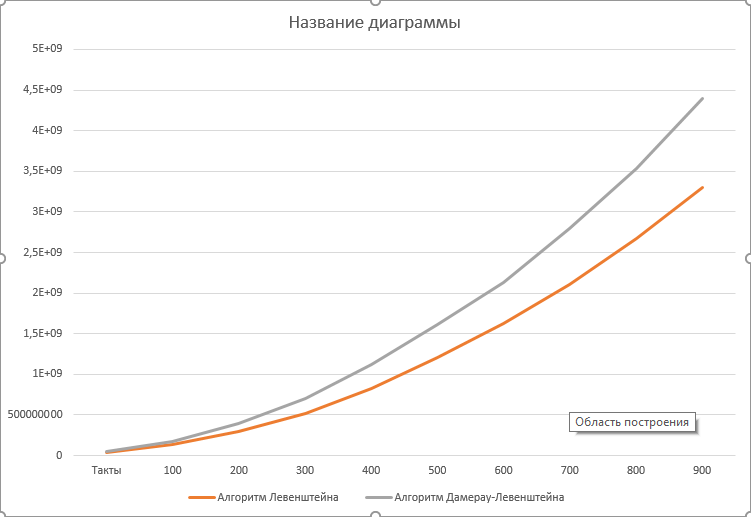
\includegraphics[width=10cm]{gr1}\\
	Рисунок 4.3.1. – график зависимости времени работы нерекурсивных алгоритмов Левенштейна и Дамерау-Левенштейна от длины входных строк 
\normalsize
\\
\\
\\
\small 
	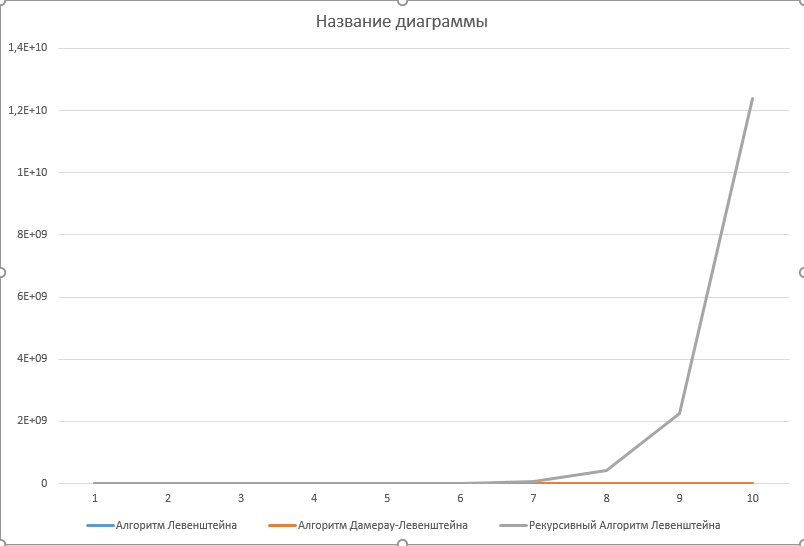
\includegraphics[width=10cm]{gr2}\\
	Рисунок 4.3.2. – график зависимости времени выполнения от длины входных строк для рекурсивного алгоритма Левенштейна 
\normalsize
\\\\

Потребление памяти программным обеспечением при выполнении рекурсивной и итеративной реализаций алгоритма Левенштейна представлено в таблице 4.2.3. На рисунках 4.2.3. и 4.2.4. представлены те же данные, но уже в виде графиков зависимостей затрачиваемой памяти от длины входных строк для нерекурсивного и рекурсивного алгоритмов соответственно.\\\\
\begin{tabular}{ | l | l | l |}
Длина строки  & Алг. Левенштейна & Рекурсивный Алг. Дамерау  \\
1 & 95821 & 94819 \\
2 & 95981 & 95966   \\
3 & 96041 & 96539 \\
4 & 96129 & 98583  \\
5 & 96185 & 114633\\
6 & 96282 & 201625 \\
7 & 96371 & 669153  \\
8 & 96501 & 3250189  \\
9 & 96589 & 17605379 \\
1 & 96635 & 97776683 \\
\end{tabular}\\
\\
\\
\small 
	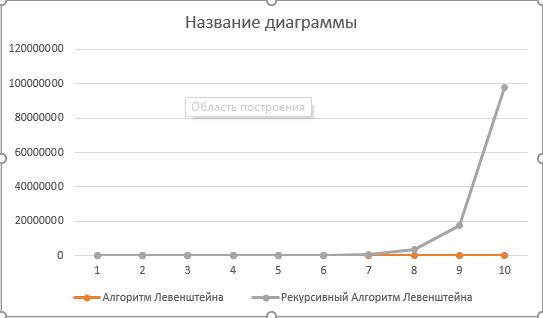
\includegraphics[width=10cm]{g3}\\
	Рисунок 4.3.3. – график зависимости памяти от длины входных строк для рекурсивного  и итеративного алгоритмов Левенштейна 
\normalsize
\\\\

\subsection{Вывод}
\label{sec:experiment:con}
На основе приведенных выше экспериментальных данных можно сделать вывод, что рекурсивная реализация алгоритма Левенштейна значительно медленнее итеративной, а их разница во времени выполнения растет вместе с ростом длины входных строк. 

\newpage
\section{Заключение}
\label{sec:finish}
В процессе выполнения лабораторной работы было проведено исследование алгоритмов Левенштейна и Дамерау-Левенштейна нахождения расстояния между строками. 
Во время разработки программного обеспечения в соответствии с поставленными требованиями были получены практические навыки реализации указанных алгоритмов: алгоритмов Левенштейна и Дамерау-Левенштейна в матричной версии и алгоритма Левенштейна в рекурсивной версии. 
При помощи разработанного программного обеспечения на материале замеров процессорного времени выполнения реализации на варьирующихся длинах строк были экспериментально подтверждены различия во временной эффективности рекурсивной и нерекурсивной версий выбранного алгоритма определения расстояния между строками. 

\newpage
\begin{thebibliography}{9}
	\bibitem 1.	В. И. Левенштейн. «Двоичные коды с исправлением выпадений, вставок и замещений символов» - М.: Доклады Академий Наук СССР, 1965.
	\bibitem 2.	Д. С. Карахтанов. «Программная реализация алгоритма Левенштейна для устранения опечаток в записях баз данных» [Электронный ресурс] / Молодой ученый. 	
                       – Режим доступа: https://moluch.ru/archive/19/1966/, свободный. (Дата обращения: 10.09.2018 г.)
	\bibitem 3.	«Метод динамического программирования Вагнера и Фишера» [Электронный ресурс] / Алгоритмы, методы, исходники. – Режим доступа: http://algolist.manual.ru/search/lcs/vagner.php, свободный. 
        (Дата обращения: 29.10.2018 г.)
	\bibitem 4. «Cтандарт С11»  – Режим доступа: http://www.open-std.org
        (Дата обращения: 29.10.2018 г.)
  
\end{thebibliography}

\end{document}